\section{Problem Definition: Proof Repair}
\label{sec:key1}

\toolname is a tool for \textit{proof repair}.
Proof repair is the problem of updating a broken proof in response to a change in a program or specification~\cite{PGL-045, pumpkinpatch}.
We can view this as a form of 
\textit{proof reuse}~\cite{Ringer2019, felty1994generalization, caplan1995logical, pons2000generalization, johnsen2004theorem}, % TODO consider citation list
or reusing proofs about one specification (say, from another library, or from within the same proof development)
to derive proofs about another specification.
The difference is that in standard proof reuse, both of these specifications continue to exist.
In contrast, proof repair is the process of reusing proofs across \textit{two versions of a single specification},
only one of which---the new version---must continue to exist.
That is, the old version of the specification may be removed after updating proofs to use the new version.

\begin{quote}
\textbf{Insight 1}:
Proof repair is a form of proof reuse---reusing proofs about one specification to derive proofs about another specification---with 
the additional challenge that one of the specifications may cease to exist (Section~\ref{sec:repair}).
The key to supporting proof repair is to build a proof reuse
tool that can handle that additional challenge (Section~\ref{sec:time}).
\end{quote}

\subsection{Repair is Transport with a Twist}
\label{sec:repair}

\begin{figure}
\codeauto{%
\begin{minipage}{0.48\textwidth}
\lstinputlisting[firstline=1, lastline=15]{equivproof.tex}
\end{minipage}
\hfill
\begin{minipage}{0.48\textwidth}
\lstinputlisting[firstline=17, lastline=32]{equivproof.tex}
\end{minipage}}
\vspace{-0.3cm}
\caption{Two functions between \lstinline{Old.list} and \lstinline{New.list} (top) that form an equivalence (bottom).}
\label{fig:equivalence}
\end{figure}

Proof repair corresponds to a particular kind of proof reuse called \textit{transport},
with the twist that the specification about which we are reusing proofs may cease to exist.
Transport is proof reuse across \textit{type equivalences}~\cite{univalent2013homotopy},
or pairs of functions that map between two types and are mutual inverses.
Figure~\ref{fig:equivalence} shows a type equivalence between the two versions of \lstinline{list}
from Section~\ref{sec:overview}, Figure~\ref{fig:listswap} that \toolname discovered and proved automatically.
When such a type equivalence between two types exists, we say those types are \textit{equivalent} (denoted $\simeq$), for example:

\begin{lstlisting}
Old.list $\simeq$ New.list
\end{lstlisting}

A transport method takes an input term $t$ and produces an output term $t'$ that is \textit{equal up to transport}
along an equivalence $A \simeq B$ (denoted $t \equiv_{A \simeq B} t'$).
Informally, equality up to transport means that if $t$ is a function, then $t'$ behaves the same way modulo the equivalence;
if $t$ is a proof, then $t'$ proves the same theorem the same way modulo the equivalence.
For example, in Section~\ref{sec:overview}, the original append function \lstinline{++} over \lstinline{Old.list}
and the updated append function \lstinline{++} over \lstinline{New.list} that \toolname produces are
equal up to transport along the equivalence from Figure~\ref{fig:equivalence}, since:

\begin{lstlisting}
$\forall$ T (l1 l2 : Old.list T), swap T (l1 ++ l2) = (swap T l1) ++ (swap T l2).
\end{lstlisting}
by induction and rewriting, and similarly in the opposite direction.
The original \lstinline{rev_app_distr} is equal to the transformed proof along the same equivalence,
since it proves the same thing the same way as the transformed proof up to the same equivalence, and up to the changes in \lstinline{++}
and \lstinline{rev}.

The formal details of equality up to transport in a univalent type theory can be found in \citet{univalent2013homotopy}, and an approximation in Coq without univalence can be found in \citet{tabareau2017equivalences}.
Note that for any equivalent \A and \B, there can be many equivalences $A \simeq B$.
Equality up to transport is along a \textit{particular} equivalence, though we erase this in the notation.

Transport methods typically work by explicitly applying the functions that make up the equivalence to convert
inputs and outputs back and forth between equivalent types.
This approach would not work for repair, since it does not make it possible to remove the old specification.
The goal of a proof repair tool like \toolname is to define a transport method that
can remove references to the old specification, %rather than converting back and forth like standard transport methods.
%That way, the proof repair tool can produce proofs that no longer refer in any way to the old specification,
since the old specification may no longer exist.

Section~\ref{sec:overview} showed a simple case of this: \toolname
reused the proof of \lstinline{rev_app_distr} defined over \lstinline{Old.list}
to generate a new proof of \lstinline{rev_app_distr} defined over equivalent \lstinline{New.list}.
Furthermore, it did so in a way that removed all references to \lstinline{Old.list}, both in the proof
and in its dependencies.
That way, after calling \lstinline{Repair}, \lstinline{Old.list} could be removed.

\begin{figure}
\begin{minipage}{0.40\textwidth}
   \lstinputlisting[firstline=1, lastline=4]{listtovect.tex}
\end{minipage}
\hfill
\begin{minipage}{0.58\textwidth}
   \lstinputlisting[firstline=6, lastline=9]{listtovect.tex}
\end{minipage}
\vspace{-0.3cm}
\caption{A vector (right) is a list (left) indexed by its length.}
\label{fig:listtovect}
\end{figure}

Viewing repair as transport is flexible enough to support changes in which the proof engineer adds or removes information.
In that case, the equivalence along which the tool transports functions and proofs
is an equivalence between \textit{refinements} ($\Sigma$ types).
It is up to the proof engineer to supply the additional information in order to construct proofs about the refinement.
Consider an example from the proof reuse tool \textsc{Devoid}~\cite{Ringer2019}:
changing a list to a length-indexed vector (Figure~\ref{fig:listtovect}).
Both \textsc{Devoid} and \toolname can repair proofs about lists to proofs about \textit{vectors of some length}, since:

\begin{lstlisting}
list T $\simeq$ $\Sigma$ (n : nat) . vector T n.
\end{lstlisting}
This is enough to automatically repair a lemma about lists:

\begin{lstlisting}
$\forall$ {A B} (l1 : list A) (l2 : list B),(@\vspace{-0.04cm}@)
  zip_with pair l1 l2 = zip l1 l2.
\end{lstlisting}
to a lemma about vectors of some length:

\begin{lstlisting}
$\forall$ {A B} (l1 : (@\codediff{$\Sigma$(n : nat).vector A n}@)) (l2 : (@\codediff{$\Sigma$(n : nat).vector B n}@)),(@\vspace{-0.04cm}@)
  zip_with pair l1 l2 = zip l1 l2.
\end{lstlisting}
recursively updating dependencies \lstinline{zip} and \lstinline{zip_with}.
It is not enough, however, to help the proof engineer get from that to a proof about vectors \textit{of a particular length}:

\begin{lstlisting}
$\forall$ {A B} (@\codediff{n}@) (l1 : (@\codediff{vector A n}@)) (l2 : (@\codediff{vector B n}@)),(@\vspace{-0.04cm}@)
  zip_with pair (@\codediff{n}@) l1 l2 = zip (@\codediff{n}@) l1 l2.
\end{lstlisting}

\textsc{Devoid} leaves this step to the proof engineer.
\toolname, in contrast, can handle this step as well.
The key is to transport functions and proofs across this equivalence:

\begin{lstlisting}
$\Sigma$(l : list T).length l = n $\simeq$ vector T n.
\end{lstlisting}
Practically, when the proof engineer changes specifications to refer to \lstinline{vector} instead of \lstinline{list},
to fix her functions and proofs, she must additionally prove invariants about the lengths of her lists (see Section~\ref{sec:dep}).
\toolname makes it easy to separate out that proof obligation, then automates the rest.

\subsection{\textsc{Carrot}: A Tool for Proof Repair}
\label{sec:time}

\begin{figure}
\begin{minipage}{0.52\textwidth}
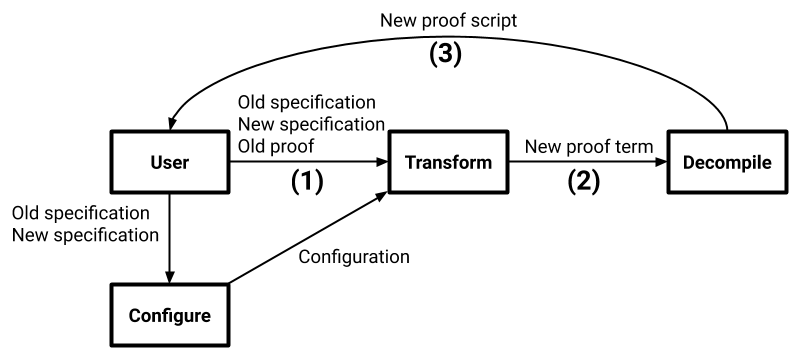
\includegraphics[width=\linewidth]{workflowa.pdf}
\end{minipage}
\hfill
\begin{minipage}{0.45\textwidth}
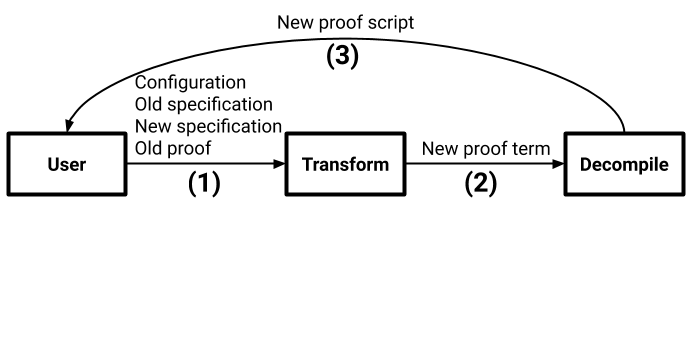
\includegraphics[width=\linewidth]{workflowb.pdf}
\vspace{0.97cm}
\end{minipage}
\vspace{-0.4cm}
\caption{The two possible workflows for \toolname, using either automatic (left) or manual (right) configuration.}
\label{fig:system}
\end{figure}

\toolname implements this transport with a twist using a proof term transformation.
The proof term transformation implements transport across equivalences,
but in a way that replaces references to the old specification (in Section~\ref{sec:overview}, the theorem that refers to \lstinline{Old.list})
with references to the new specification (in Section~\ref{sec:overview}, the theorem that refers to \lstinline{New.list}).
This proof term transformation is configurable to a particular equivalence:
it takes a \textit{configuration} (see Section~\ref{sec:configurable}) 
that tells \toolname how to transform certain constructors, eliminators, and equalities that 
correspond to the equivalence.
The configuration can be supplied manually, or discovered automatically by a search procedure.

Figure~\ref{fig:system} shows how this comes together when the proof engineer invokes \toolname:

\begin{enumerate}
\item \toolname configures itself, either:
\begin{enumerate}
\item automatically (left), using \textbf{Configure} to discover the configuration, or
\item manually (right), by taking the configuration as an argument.
\end{enumerate}
\item The configured \textbf{Transform} transforms the old proof term into the new proof term.
\item \textbf{Decompile} produces a new proof script from the new proof term.
\end{enumerate}

The example in Section~\ref{sec:overview} uses automatic configuration. When we run the \lstinline{Repair} command,
\textbf{Configure} invokes a search procedure that automatically proves the equivalence in Figure~\ref{fig:equivalence},
then configures \textbf{Transform} using that equivalence.
\textbf{Transform} then ports the proof term that inducted over \lstinline{Old.list}
to induct over \lstinline{New.list}, and finally
\textbf{Decompile} produces the tactic script in Figure~\ref{fig:auto}.

There are currently four search procedures for automatic configuration implemented in \toolname:
one for porting tuples to records, two for porting non-dependent types to certain dependent types, 
and one for permuting and renaming constructors.
All of these are informed by the needs of real proof engineers.
Manual configuration makes it possible for the proof engineer to directly configure the tool to a particular equivalence
for which no search procedure is yet implemented.
Section~\ref{sec:search} shows examples of both workflows as applied to real proof reuse and repair scenarios.




